% geDIG Paper Restructured Draft (2025-09)
% Use pdftex driver (remove uplatex/dvipdfmx to avoid driver mismatch under pdflatex)
\documentclass[ja=standard,lualatex]{bxjsarticle}
\usepackage{amsmath,amssymb,graphicx,booktabs}
% Algorithms for pseudocode
\usepackage{algorithm}
\usepackage{algpseudocode}
\usepackage{tikz}
\usepackage{float}
\usetikzlibrary{arrows.meta,positioning,calc}
% Make figure path robust
% Allow graphics both when compiling from project root or from docs/paper
\graphicspath{{figures/}{docs/paper/figures/}}
\usepackage{hyperref}
\usepackage{enumitem}

\title{geDIG: 単一スカラーで学習と推論を同時運転する動的知識構造管理}
\author{宮内 和義}
\date{2025年9月16日 草稿案}

\begin{document}
\maketitle

\begin{abstract}
本稿は,知識グラフの構造統合($\Delta\mathrm{GED}$)と情報整理($\Delta\mathrm{IG}$)を単一スカラー
$\mathcal{F}=\Delta\mathrm{GED}_{\mathrm{norm}}-\lambda\,\Delta\mathrm{IG}_{\mathrm{norm}}$ に統合し,学習と推論を同時運転するための洞察イベント検出器 geDIG を提示する。主な貢献は次のとおり:
(1)\textbf{One‑Gauge 運用}: $\mathcal{F}<\theta_{\mathrm{event}}$ を洞察イベントとして検出し,探索・配線・バックトラック・メモリエビクションを\emph{同一基準}でイベント駆動制御。
(2)\textbf{理論整合の補題}: 正規化・上界化・比例定数吸収の前提下で $\mathcal{F}\propto\Delta\mathrm{MDL}$(FEP/MDL 橋渡し)の操作的整合を提示。
(3)\textbf{横断実験}: 部分観測迷路でステップ数 $-25.8$\% を達成し,RAG でプロンプト強化率 167.7\%・受容率 100\% を確認。
(4)\textbf{実運用性と限界}: しきい値の分位校正・多ホップ($H{=}3$)で 100--320ms 級を実測し,再現スクリプトと校正アーティファクトを含むパッケージ,および限界(IG 定義感度/集約設計/スケール)を明記。
本稿は geDIG を理論の強主張ではなく\,\emph{運用ヒューリスティック}(operational gauge)として提示する。
\end{abstract}

% Quick primer box removed (moved to a light note under the terminology table)

% (English abstract removed; Japanese abstract incorporates the same conservative content.)

\section{はじめに}
私たちが「ひらめいた」と感じる瞬間には、散らばっていた経験や知識が\emph{構造としてつながり}、同時に\emph{意味の秩序が立ち上がる}。この感覚は近年の脳科学でも、海馬における\textit{リプレイ}(Hippocampal Replay)として、覚醒時・睡眠時に体験系列が順・逆に再生される現象として報告されている\,\cite{Buzsaki2015,Carr2011,Pfeiffer2013}。本稿は、この\textbf{同時性}を動的に成長する知識グラフ上で可観測にし、\textbf{学習(記憶の整理)と推論(探索・検索)の同時展開}、および\textbf{動的知識グラフの管理}という洞察生成に不可欠な二要件を、単一スカラーの計器で運用可能にする枠組み geDIG を提示する。

具体的には、知識グラフの\textbf{構造統合}(正規化グラフ編集距離の減少)と\textbf{情報整理}(エントロピー低下)を
\begin{equation*}
  \mathcal{F} = \Delta\mathrm{GED}_{\mathrm{norm}} - \lambda\,\Delta\mathrm{IG}_{\mathrm{norm}}
\end{equation*}
 に統合し、$\mathcal{F}<\theta$ を\textbf{洞察イベント}として検出する。geDIG 値 $\mathcal{F}$ をイベント駆動信号として用いることで、\textbf{探索深さ・候補幅・バックトラック・メモリエビクション}までを\textit{同一基準}で横断制御できる(図\ref{fig:overview})。

\paragraph{記号と正規化(実装準拠)} 構造項 $\Delta\mathrm{GED}_{\mathrm{norm}}$ は,ノード/エッジ編集コストの和を\textbf{総和規格化} $(n_1{+}n_2{+}e_1{+}e_2)\cdot\max\{c_\mathrm{node},c_\mathrm{edge}\}$ で割った値に基づく\textbf{構造改善} $\mathrm{SI}\in[-1,1]$($-\,\mathrm{GED}_{\mathrm{norm}}$ とグラフ効率指標の線形結合,必要に応じてスペクトル補助)を用いる.意思決定時には\textbf{局所正規化}(Layer1 候補数 $K$ に対する $C_{\max}^{\mathrm{local}}{=}1{+}K$)を用いる場合がある.情報項 $\Delta\mathrm{IG}$ は\textbf{局所エントロピーの分散低下}により定義する(各ノード近傍の埋め込み類似度から確率を構成し Shannon エントロピーを計算,その分散の before→after 低下量).IG は\texttt{raw}/\texttt{z}(z-score)/\texttt{norm}($\tanh$ 正規化)で運用でき,必要に応じて非負クラップ(負の IG を 0 とみなす)を適用する.最終結合は $\mathcal{F}=\mathrm{SI}-\lambda\,\mathrm{IG}$(実装の \texttt{lambda\_weight})で与える.

\noindent\textit{記号と既定(要約)}: 本文の式に対応する主要記号を表に整理する(レンジは本文に現れる代表例)。
\begin{table}[H]
\centering
\small
\begin{tabular}{ll}
\toprule
記号 & 定義/レンジ(参考) \\
\midrule
$\mathcal{F}$ & $\Delta\mathrm{GED}_{\mathrm{norm}}-\lambda\,\Delta\mathrm{IG}_{\mathrm{norm}}$\\
$g_0$ & 0-hop の geDIG 値(FEP/誤差寄り)\\
$g_{\min}$ & multi-hop の最小 geDIG 値(MDL/短絡寄り)\\
$b(t)$ & 二段ゲートの集約値:$b(t){=}\min\{g_0, g_{\min}\}$(NA 発火時)\\
$\theta_{\mathrm{NA}}$ & NA ゲート閾値(例:$[-5.5,-4.5]\times10^{-3}$;式\,\ref{eq:na_trigger})\\
$\theta_{\mathrm{BT}}$ & BT ゲート閾値(例:$[-1.4,-1.0]\times10^{-2}$;式\,\ref{eq:na_da_gate})\\
$H,\,\gamma$ & 多ホップ段数と減衰(例:$H{=}3$, $\gamma\approx 0.9$)\\
$\lambda$ & 構造/情報の相対重み($\approx c_D/c_M$;分位校正と併用)\\
\bottomrule
\end{tabular}
\end{table}

\paragraph{符号規約と閾値} geDIG は\emph{コスト}として解釈し,\textbf{小さいほど良い}(最小化対象).更新候補の評価は $\Delta\mathcal{F}=\mathcal{F}_{\mathrm{after}}-\mathcal{F}_{\mathrm{before}}$ とし,$\Delta\mathcal{F}< -\tau$ で\textbf{受容}(追加),$\Delta\mathcal{F}>+\tau$ で\textbf{圧縮/見直し}とする.スパイク判定は構成パラメタ(例:$\theta_{\mathrm{NA}},\theta_{\mathrm{BT}}$)と併用し,$\lambda$($k$)はタスク/ホップで校正可能である.

\begin{figure}[H]
  \centering
  \includegraphics[width=0.92\linewidth]{fig5_concept_new}
  \caption{geDIG のコンセプト図。構造統合($\Delta$GED)と情報整理($\Delta$IG)を単一スカラー $\mathcal{F}$ に統合し、検出→制御に直結させる。}
\label{fig:concept}
\end{figure}

\paragraph{前提と上界($\mathcal{F}\propto\Delta\mathrm{MDL}$ の実運用仮定)}
本稿では $\mathcal{F}=\mathrm{SI}-\lambda\,\mathrm{IG}$ を差分MDLに比例する\,\emph{運用ゲージ}として扱う。査読耐性のために前提を本文に明記する。(i)\textbf{正規化}: 編集コストは総和規格化(ノード/エッジ数と単価の上限)し,IG は局所エントロピーの分散低下を $\log d$ などの上限で無次元化する。(ii)\textbf{置換の上界化}: 構造の置換は削除+挿入の和で上界化し,GED の差分で近似する。(iii)\textbf{比例定数の吸収}: モデル記述長とデータ記述長の単位差は $\lambda$ に吸収し,\,$k{=}\lambda$ の校正で実験ごとに整合させる。(iv)\textbf{誤差項の扱い}: 高次項とスペクトル補助は $\varepsilon$ としてまとめ,multi-hop の有限和($H{=}3$)で上界を評価する。以上の前提下で $\Delta\mathrm{MDL}\approx c_M\,\Delta\mathrm{GED}_{\mathrm{norm}}-c_D\,\Delta\mathrm{IG}_{\mathrm{norm}}$ と見なし,$\lambda\approx c_D/c_M$ により $\mathcal{F}\propto\Delta\mathrm{MDL}$ と運用する(詳細は付録A)。



\subsection*{用語対応表(式 \,$\leftrightarrow$\, 実装)}
\begin{table}[H]
\centering
\small
\begin{tabular}{ll}
\toprule
理論表現 & 実装(主なフィールド/パラメタ)\\
\midrule
$\mathcal{F}$(geDIG) & \texttt{GeDIGResult.gedig\_value}\\
$\mathrm{SI}$(構造改善) & \texttt{GeDIGResult.structural\_improvement},\texttt{normalized\_ged()}\\
$\mathrm{IG}$(情報利得) & \texttt{GeDIGResult.ig\_value}/\texttt{ig\_z\_score}(\texttt{ig\_mode})\\
$\lambda$(k) & \texttt{GeDIGCore.lambda\_weight}\\
$\tau$(受容閾値) & 運用基準($\Delta\mathcal{F}$);監視系は \texttt{tau\_s},\,\texttt{tau\_i}\\
スパイク閾値 & \texttt{GeDIGCore.spike\_threshold}(閾値モード時)\\
0/多ホップ設定 & \texttt{enable\_multihop, max\_hops, decay\_factor}\\
SP利得 & \texttt{use\_multihop\_sp\_gain},\,\texttt{sp\_norm\_mode}(relative)\\
局所正規化 & \texttt{use\_local\_normalization}($C_{\max}^{\mathrm{local}}{=}1{+}K$)\\
効率/スペクトル & \texttt{efficiency\_weight},\,\texttt{enable\_spectral},\,\texttt{spectral\_weight}\\
\bottomrule
\end{tabular}
\caption{式と実装の対応。詳細は \texttt{algorithms/gedig\_core.py} および \texttt{algorithms/core/metrics.py} を参照。}
\end{table}

% Light quick pointers (moved from top; keep tone neutral)
\vspace{0.5ex}
{\footnotesize
\textit{補助メモ(運用の勘どころ)}:
\begin{itemize}[leftmargin=1.1em, itemsep=0.15em]
  \item geDIG はコスト最小化(小さいほど良い):$\mathcal{F}=\mathrm{SI}-\lambda\,\mathrm{IG}$
  \item 受容/圧縮の目安:$\Delta\mathcal{F}<{-}\tau$ は追加、$\Delta\mathcal{F}>{+}\tau$ は圧縮
  \item IG は局所エントロピー分散の低下(raw / z / $\tanh$)で運用
  \item 実験運用は 校正→固定→本番($k{=}\lambda$, $\tau$, $\tau_{\mathrm{bt}}$)
\end{itemize}
}

% L0–L4 全体像(update_2025_09 と同配線・レイアウト)
\begin{figure}[H]
  \centering
  \resizebox{0.95\linewidth}{!}{%
  \begin{tikzpicture}[>=latex, node distance=5mm]
    % Layers
    \node[draw, rounded corners, align=center, inner sep=3mm, fill=blue!5, minimum width=9.5cm] (l0) {L0(入力):感覚皮質/視覚野(埋め込み・エンコーディング,任意)};
    \node[draw, rounded corners, align=center, inner sep=3mm, fill=green!5, below=3mm of l0, minimum width=9.5cm] (l1) {L1(小脳):誤差検出(探索トリガ)};
    \node[draw, rounded corners, align=center, inner sep=3mm, fill=yellow!10, below=3mm of l1, minimum width=9.5cm] (l2) {L2(海馬):エピソード記憶と検索(RAG)};
    \node[draw, rounded corners, align=center, inner sep=3mm, fill=orange!10, below=3mm of l2, minimum width=9.5cm] (l3) {L3(前頭前野):GNN統合+geDIG($\Delta$GED/$\Delta$IG)+矛盾検出};
    \node[draw, rounded corners, align=center, inner sep=3mm, fill=red!5, below=3mm of l3, minimum width=9.5cm] (l4) {L4(言語野):LLM応答生成(外部フィードバック取り込み)};
    % geDIG sensor badge
    \node[draw, rounded corners, inner sep=1mm, fill=white, below=1mm of l3] (badge) {\footnotesize geDIG $\mathcal{F}<\theta$(洞察イベント)};
    % Arrows
    \draw[->] (l0) -- (l1);
    \draw[->] (l1) -- (l2);
    \draw[->] (l2) -- (l3);
    \draw[->] (l3) -- (l4);
    % Control feedback
    \draw[->, dashed] (l3.west) .. controls +(-2,0.5) and +(-2,-0.5) .. node[left, align=center] {イベント駆動制御\\(取得段数/候補幅/BT/エビクション)} (l2.west);
  \end{tikzpicture}%
  }
  \vspace{0.8ex}
  \caption{全体像(L0〜L4):L3に配置されたgeDIGセンサーが洞察イベントを検出し、L2/L4の動作をイベント駆動で横断制御する。}
  \label{fig:overall-architecture}
\end{figure}

\noindent\textit{補足(集約の合理性)}: $b(t){=}\min\{g_0,g_{\min}\}$ は保守的(過少評価)な集約であり,偽橋や偶然接続の過検出を抑制するための選択である.代替として soft-min(温度 $\tau$)や加重和も運用可能である:\,$\operatorname{softmin}_\tau(x,y){=}-\tau\log\big( e^{-x/\tau}{+}e^{-y/\tau} \big)$.本稿では偽陽性率の管理を優先して \texttt{min} を採用し,soft-min 等は限界と今後の課題で比較を提案する.

\subsection*{研究目的}
本研究の目的は、洞察を「\emph{構造統合と情報整理の同時発生}」として操作化し、geDIG 値 $\mathcal{F}$ によって\textbf{(i) 学習×推論の同時展開}と\textbf{(ii) 動的知識グラフの管理}を\textbf{同一の運用規約}で実現できることを、理論整合と実験で示すことである。理論面では、差分MDL/自由エネルギー原理との比例関係(定数因子内)を補題として与え、0-hop=FEP 寄り/h-hop=MDL 寄りという運用解釈を明確にする。

\subsection*{タスク設定と検証範囲}
上記二要件を現実系で検証するために、二つの代表タスクを設定した。\textbf{部分観測迷路}では、地図を\emph{作りながら}進む設定で $\mathcal{F}<\theta$ をトリガに配線採否・バックトラック等を制御する。\textbf{オンライン更新 RAG} では、同じ $\mathcal{F}$ を検索深さ・サブグラフ・メモリエビクションに適用し、多ホップ合成で遠距離の橋を評価する。

% [Removed] 重複していた「本稿/本研究の貢献」節は一旦削除(要約は Abstract/導入に統合)

\section{理論: 学習と推論の同時運転}
\subsection{設計指針(R1--R4)}
以下は本稿で採用した設計上の指針の要約であり、要件というより設計のねらいを簡潔に示す。
\textbf{R1: 共通スケール化}. 構造(GED)と情報(IG)を無次元化し、同一スケールで比較可能とする($\Delta\mathrm{GED}/C_{\max}$, $\Delta\mathrm{IG}/\log d$)。\quad
\textbf{R2: 逐次差分観測}. before$\to$after の差分として定義し、各ステップで即時に読めるようにする。\quad
\textbf{R3: 遠距離感度}. 短絡利得を取り込み、遠距離の橋も評価対象に含める(\S2.3)。\quad
\textbf{R4: 単一ゲージ運用}. $\mathcal{F}<\theta$ の基準で探索/配線/BT(バックトラック)/エビクションを横断的に制御する(図\ref{fig:overview})。

\subsection{計算前提:GED の計算困難性と近似戦略}
グラフ編集距離(GED)の厳密計算は一般に NP 困難である\,\cite{gao2010survey}。オンラインの\emph{検出→制御}ループに組み込むため、本研究では\textbf{クエリ中心・局所多ホップ}評価を採用する。すなわち、時刻 $t$ の\,\emph{現在クエリ} $q_t$ を焦点として、
\begin{itemize}[leftmargin=*]
  \item \textbf{0-hop ($g_0$)}: $q_t$ 近傍での編集のみを反映した正規化差分 $\Delta\mathrm{GED}_{\mathrm{norm}}$ と $\Delta\mathrm{IG}_{\mathrm{norm}}$ の組合せ。
  \item \textbf{$h$-hop ($g^{(h)}$)}: $q_t$ 周辺の $h$-近傍部分グラフに対する差分評価。$h\in\{1,\dots,H\}$ の合成により遠距離の橋(短絡利得)を拾う。
\end{itemize}
計算量は候補幅 $k$ と最大ホップ $H$ に対して概ね $O(k^H)$。実装では $H{=}3$、候補列挙幅を小さく保つことで 100--320ms 級の評価を達成する。局所正規化(例: $C^{\text{local}}_{\max}=1+K$)を併用し、各ステップ間で無次元の一貫性を確保する。以降、$g_0$ を 0-hop geDIG、$g_{\min}=\min_{1\le h\le H} g^{(h)}$ を multi-hop の最小値と呼び、二段ゲート(\S\ref{sec:na_da_gate})で用いる。



\subsection{直感から式へ:0-hop と $h$-hop}
0-hop は編集コスト(誤差)主導で曖昧さ検出に向き、$h$-hop は短絡利得(平均最短路の縮み)により実効構造コストを下げうる。最小例では、0-hop 直後は $\Delta\mathrm{GED}_{\mathrm{norm}}>0$ だが、1--2 hop で $\mathcal{F}$ が閾値を跨いでイベント化する。これが、誤差/驚き最小化(FEP)と複雑さ最小化(MDL)を単一スカラーで橋渡しできる理由である。

\begin{figure}[H]
  \centering
  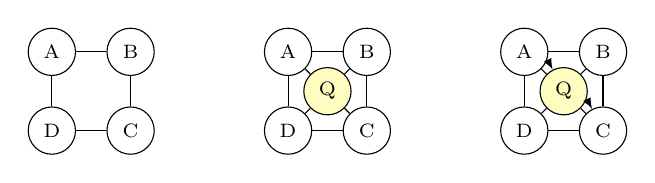
\begin{tikzpicture}[scale=1.0,
    node/.style={circle,draw,minimum size=6mm,inner sep=0pt, font=\scriptsize}]
    % --- Before (square) ---
    \node[node] (A1) at (0,1) {A};
    \node[node] (B1) at (1,1) {B};
    \node[node] (C1) at (1,0) {C};
    \node[node] (D1) at (0,0) {D};
    \draw (A1)--(B1)--(C1)--(D1)--(A1);

    % --- After (0-hop): add Q + 4 edges ---
    \node[node] (A2) at (3,1) {A};
    \node[node] (B2) at (4,1) {B};
    \node[node] (C2) at (4,0) {C};
    \node[node] (D2) at (3,0) {D};
    \draw (A2)--(B2)--(C2)--(D2)--(A2);
    \node[node, fill=yellow!25] (Q2) at (3.5,0.5) {Q};
    \draw (Q2)--(A2) (Q2)--(B2) (Q2)--(C2) (Q2)--(D2);

    % --- h=1: shortcuts reduce path length (effective cost) ---
    \node[node] (A3) at (6,1) {A};
    \node[node] (B3) at (7,1) {B};
    \node[node] (C3) at (7,0) {C};
    \node[node] (D3) at (6,0) {D};
    \draw (A3)--(B3)--(C3)--(D3)--(A3);
    \node[node, fill=yellow!25] (Q3) at (6.5,0.5) {Q};
    \draw (Q3)--(A3) (Q3)--(B3) (Q3)--(C3) (Q3)--(D3);
    \draw[dashed,->,>=latex] (A3) to[bend left=18] (Q3);
    \draw[dashed,->,>=latex] (Q3) to[bend left=18] (C3);
  \end{tikzpicture}
  \vspace{0.8ex}
  \caption{最小例(正方形グラフに中心クエリ Q を追加)。0-hop 直後は編集コストが純増するが、$h{=}1$ では短絡により平均最短路が縮み、実効構造コストが低下して $\mathcal{F}$ が閾値を跨ぎ得る。}
  \label{fig:minimal_example}
\end{figure}

\subsection{One‑Gauge によるイベント駆動制御}
図\ref{fig:overview} に示すように、geDIG センサーは FEP(誤差最小化)側と MDL(複雑さ最小化)側から情報を受け取り、
単一スカラー $\mathcal{F}$ で洞察イベントを検出する。本稿では、運用上のイベント検出は二段ゲート(NA/BT)で行い、各々の閾値を $\theta_{\mathrm{NA}}$、$\theta_{\mathrm{BT}}$ として\S\,\ref{sec:na_da_gate}(式\,\ref{eq:na_trigger}--\ref{eq:na_da_gate})に定義する。これらを総称して $\theta_{\mathrm{event}}$ と呼ぶことにする。$\mathcal{F}$ が該当閾値を跨いだとき、探索深さ・候補幅・バックトラック・メモリエビクションを即時制御する。



\begin{figure}[H]
  \centering
  \begin{tikzpicture}[>=latex, node distance=12mm]
    % Inputs
    \node[draw, rounded corners, align=center, inner sep=3mm, fill=blue!5] (fep0) {0-hop\\$g_0$(FEP/誤差)};
    \node[draw, rounded corners, align=center, inner sep=3mm, fill=green!5, right=36mm of fep0] (mdlmin) {multi-hop\\$g_{\min}$(MDL/短絡)};
    % Combine
    \node[draw, thick, rounded corners, align=center, inner sep=4mm, below=14mm of $(fep0)!0.5!(mdlmin)$, fill=gray!10] (combine) {$b(t)=\min\{\,g_0,\,g_{\min}\,\}$};
    % Threshold gates
    \node[draw, rounded corners, inner sep=2.5mm, below left=12mm and 10mm of combine, align=center] (na) {NA ゲート\\$g_0>\theta_{\mathrm{NA}}$};
    \node[draw, rounded corners, inner sep=2.5mm, below right=12mm and 10mm of combine, align=center] (bt) {BT ゲート\\$b(t)\le\theta_{\mathrm{BT}}$};
    % Optional SP
    \node[draw, rounded corners, inner sep=2mm, left=26mm of na, align=center, fill=yellow!15] (sp) {$\Delta\mathrm{SP}$ 測定\\(NA 時に強制)};
    % Control block
    \node[draw, rounded corners, inner sep=3mm, below=14mm of $(na)!0.5!(bt)$, align=center, text width=88mm] (ctrl) {イベント駆動制御:取得段数/候補幅、バックトラック、サブグラフ選択、メモリエビクション};

    % Arrows
    \draw[->] (fep0) -- (combine);
    \draw[->] (mdlmin) -- (combine);
    \draw[->, dashed] (combine) -- (na);
    \draw[->, dashed] (combine) -- (bt);
    \draw[->] (na) -- (sp);
    \draw[->] (na) -- (ctrl);
    \draw[->] (bt) -- (ctrl);
  \end{tikzpicture}
  \vspace{0.6ex}
  \caption{One‑Gauge のイベント駆動フロー。0-hop の $g_0$(FEP/誤差)と multi-hop の $g_{\min}$(MDL/短絡)を $b(t)=\min(g_0,g_{\min})$ に集約し、$\theta_{\mathrm{NA}}$・$\theta_{\mathrm{BT}}$ で制御に接続する。必要に応じて NA 時に $\Delta\mathrm{SP}$ を強制測定する。}
  \label{fig:overview}
\end{figure}

\paragraph{$\Delta\mathrm{SP}$(平均最短路差)の定義} 誘導サブグラフ $G'$ 上の平均最短路長 $\mathrm{SPL}(G')$ を用い,追加前後での差 $\Delta\mathrm{SP}=\mathrm{SPL}(G'_{\mathrm{after}})-\mathrm{SPL}(G'_{\mathrm{before}})$ を測る.$\Delta\mathrm{SP}<0$ は\textit{ショートカット}の形成を示し,$g_{\min}$ の評価補助として NA 時に強制測定する.重み付き辺のときは距離定義に応じて置換する.

% [Moved/Unified] 擬似コードは \paragraph{擬似コード(One‑Gauge 制御)} の直下に一本化

\subsection{最小ランニング例(定量・直観)}
正方形グラフ $A$-$B$-$C$-$D$ に中心ノード $Q$ を追加する例(図\,\ref{fig:minimal_example})を考える。0-hop 直後は編集コストが増え($\mathrm{GED}_{\mathrm{norm}}{>}0$),グラフ効率の上昇を加味しても $\mathrm{SI}{<}0$ になりやすい。一方,$h{=}1$ ではショートカットにより\,\textit{実効コストが低下}し,$\mathrm{SI}$ が改善する。情報項 IG は近傍の類似度構造が整理されると正となる(分散低下)。

\begin{table}[H]
\centering
\small
\begin{tabular}{lrrrrr}
\toprule
状態 & $\mathrm{GED}_{\mathrm{norm}}$ & $\Delta \mathrm{Eff}$ & $\mathrm{SI}$ & $\mathrm{IG}$ & $\mathcal{F}{=}\mathrm{SI}{-}\lambda\,\mathrm{IG}$\\
\midrule
基準(正方形) & $0$ & $-$ & $0$ & $-$ & $0$\\
0-hop:$Q$ 追加 & $\approx 0.24$ & $+0.10$ & $\approx -0.14$ & $>0$ & $<0$\\
1-hop:短絡反映 & $\downarrow$ & $+\,$(維持) & $\uparrow\,\,(\gtrsim 0)$ & $>0$ & $\lesssim 0$\\
\bottomrule
\end{tabular}
\caption{最小例の挙動(例値; $\lambda$ 小さめ)。短絡で $\mathrm{SI}$ が回復し,IG も正なら $\mathcal{F}$ が閾値を跨ぎ得る。}
\end{table}

\noindent 注: $\mathrm{SI}$ は $-\mathrm{GED}_{\mathrm{norm}}$ とグラフ効率(必要に応じてスペクトル)の線形結合。IG は局所エントロピー分散の低下量(raw/z/\,$\tanh$)。

\subsection{差分MDL/FEPとの対応}
$\Delta\mathrm{GED}_{\mathrm{norm}}=\mathrm{GED}/C_{\max}$、$\Delta\mathrm{IG}_{\mathrm{norm}}=(H(\mathbf{v}_{t-1})-H(\mathbf{v}_t))/\log d$ と定義し、
正規化により $\mathcal{F}$ は無次元量となる。$\mathcal{F}$ は以下に比例する。
\begin{equation}
  \Delta \mathrm{MDL} \approx c_M\,\Delta\mathrm{GED}_{\mathrm{norm}} - c_D\,\Delta\mathrm{IG}_{\mathrm{norm}} \propto \mathcal{F}
\end{equation}
差分MDL の境界を跨ぐとき $\mathcal{F}<\theta$ となり、探索と記憶の臨界運用(Edge-of-Insight)が実現する。

\paragraph{命題1(運用比例・十分条件,証明スケッチ)}\label{prop:operational_mdl} 記述長 $\mathrm{MDL}(M,D)=L(M)+L(D\mid M)$ を構造コスト $L(M)\approx c_M\,\Delta\mathrm{GED}_{\mathrm{norm}}$、データ符号長 $L(D\mid M)\approx c_D\,(1-\Delta\mathrm{IG}_{\mathrm{norm}})$ で1次近似すると、差分は(cf.~MDL:\,\cite{rissanen1978};FEP:\,\cite{Friston2010})
\begin{align}
  \Delta \mathrm{MDL} &\approx c_M\,\Delta\mathrm{GED}_{\mathrm{norm}} - c_D\,\Delta\mathrm{IG}_{\mathrm{norm}} + \text{const.}
\end{align}
となる。比例係数 $\lambda=c_D/c_M$ を選べば $\mathcal{F}=\Delta\mathrm{GED}_{\mathrm{norm}}-\lambda\,\Delta\mathrm{IG}\ \propto\ \Delta \mathrm{MDL}$。ここで $\Delta\mathrm{GED}_{\mathrm{norm}}$ は総和規格化に基づく $[-1,1]$ 近傍の値,$\Delta\mathrm{IG}$ は分散低下(raw)を\,z-score もしくは $\tanh$ で正規化して用いる(実装切替可)。削除+挿入による上界化と比例定数の閾値吸収を前提とする。\textbf{本命題は等価主張ではなく,運用上の比例(定数因子内)を与える}。十分条件と誤差上界は本文に集約し,付録Aは補助とする。

\noindent\textit{本文内の前提と上界の要約}(詳細は\S\,\ref{sec:na_da_gate}, 付録A):
\begin{itemize}[leftmargin=*]
  \item 正規化: $\Delta\mathrm{GED}$ は総和規格化,$\Delta\mathrm{IG}$ は $\log d$ 等で無次元化(\S1.1)。
  \item 置換の上界化: 構造置換は削除+挿入の和で上界化(GED 差分近似)。
  \item 比例定数の吸収: 単位差は $\lambda\,{=}\,c_D/c_M$ に吸収(分位校正と併用)。
  \item 多ホップ有限和: 合成誤差は $\epsilon\le \frac{(1+\lambda)\,\gamma^{H}}{1-\gamma}$(式\,\eqref{eq:multi_err})。
\end{itemize}

\begin{figure}[t]
  \centering
  \begin{tikzpicture}[>=latex, node distance=12mm]
    \node[draw, rounded corners, align=center, inner sep=3mm] (fep) {FEP側\\(誤差/驚き 最小化)};
    \node[draw, rounded corners, align=center, inner sep=3mm, right=30mm of fep] (mdl) {MDL側\\(構造/複雑さ 最小化)};
    \node[draw, thick, rounded corners, align=center, inner sep=4mm, below=14mm of $(fep)!0.5!(mdl)$, fill=gray!10] (gedig) {geDIG(差分・オンライン・単一スカラー)\\$\mathcal{F}=\Delta\mathrm{GED}_{\text{norm}}-\lambda\,\Delta\mathrm{IG}_{\text{norm}}$};
    \node[draw, rounded corners, align=center, inner sep=3mm, below=14mm of gedig] (event) {洞察イベント検出($\mathcal{F}<\theta$)};
    \node[draw, rounded corners, align=center, inner sep=3mm, below=14mm of event, text width=72mm] (control) {イベント駆動制御:\\取得段数/候補幅、バックトラック、サブグラフ選択、\\メモリエビクション(RAG/探索/記憶を横断)};
    \draw[->] (fep.south) -- ++(0,-6mm) -| (gedig.north west);
    \draw[->] (mdl.south) -- ++(0,-6mm) -| (gedig.north east);
    \draw[->] (gedig) -- (event);
    \draw[->] (event) -- (control);
  \end{tikzpicture}
  \vspace{0.8ex}
  \caption{FEP–MDL 二軸を単一スカラー $\mathcal{F}$ に写像し、$\mathcal{F}<\theta$ を洞察イベントとして検出、RAG/探索/記憶の即時制御に直結する全体配線。}
  \label{fig:fep_mdl_bridge}
\end{figure}

\subsection{多ホップ合成と短絡利得}
 多ホップ合成は式\eqref{eq:multi_hop} のように定義する。
\begin{equation}
  \mathcal{F}^{\text{multi}}_t = \sum_{h=1}^{H} \gamma^{h-1} \Big( \Delta\mathrm{GED}^{(h)}_{\mathrm{eff}} - \lambda\,\Delta\mathrm{IG}^{(h)}_{\mathrm{norm}} \Big)
  \label{eq:multi_hop}
\end{equation}
ここで $\Delta\mathrm{GED}^{(h)}_{\mathrm{eff}} = \Delta\mathrm{GED}_{\mathrm{norm}} - \Delta\mathrm{SP}^{(h)}_{\mathrm{norm}}$ は短絡利得を差し引いた実効コストである。有限和近似の切り捨て誤差は幾何級数の評価から
\begin{equation}
  \epsilon \le \frac{(1+\lambda)\,\gamma^{H}}{1-\gamma}\,.
  \label{eq:multi_err}
\end{equation}
許容誤差 $\tau$ に対し、
\begin{equation}
  H \;\ge\; \left\lceil \frac{\log\big(\tau(1-\gamma)/(1+\lambda)\big)}{\log \gamma} \right\rceil
\end{equation}
 が十分条件となる。例えば $\gamma{=}0.9,\;\lambda{\approx}1,\;\tau{=}0.1$ なら \,$H{=}3$\,で十分小さい。実装と実測(100--320ms)でも $H{=}3$ は実用的である。
\paragraph{0-hop の IG 定義(実装要約)}
エントロピー $H(\mathbf{v}_t)$ は、エピソードベクトル $\mathbf{v}$ の各成分をカテゴリ(one-hot)またはビン化(連続)で離散化した結合分布の近似から計算し、\,$\Delta\mathrm{IG}_{\mathrm{norm}}=(H(\mathbf{v}_{t-1})-H(\mathbf{v}_t))/\log d$\,で正規化する。ここで $d$ は有効状態の語彙サイズで、実装では局所辞書の更新に追随して逐次推定する(RAG/迷路で共通運用)。
\paragraph{0-hop と multi-hop の役割}
0-hop は仮配線直後の構造編集コストを評価し、FEP 的な“誤差/曖昧さ”の検出器として機能する。一方で $h\ge1$ の multi-hop 評価は、短絡(平均最短路の縮み)を通じて MDL 的な“複雑さ削減”を捉える。実装では $g_0$ が NA 的注意のトリガとなり、multi-hop の最小 $g_{\min}$ が DA 的価値信号として解釈される(定義は\S\ref{sec:na_da_gate})。この二層構造により、曖昧さの検知と短絡の評価が同一ステップで連鎖する。

\subsection{二段ゲート(NA/DA)と操作的対応}\label{sec:na_da_gate}
0-hop の geDIG を $g_0(t)$、multi-hop 評価の最小値を $g_{\min}(t):=\min_{1\le h\le H} \mathcal{F}^{(h)}_t$ と定義する。$g_0$ がゼロ近傍に滞留している局面は、直近の仮配線で構造成長が乏しく曖昧さ(不確実性)が高い状態を意味する。本稿ではこれをノルアドレナリン(NA)的な注意・探索の立ち上がりに対応づける操作的仮説\,(cf.~\cite{AstonJones2005})として用い、次式の二段ゲートを定義する。
\begin{equation}
  \mathrm{NA}(t) := \mathbb{I}[\, g_0(t) > \theta_{\mathrm{NA}}\,],\qquad \theta_{\mathrm{NA}}\in[-5.5,-4.5]\times10^{-3}.
  \label{eq:na_trigger}
\end{equation}
NA が発火したフレームでは multi-hop の短絡(負側)を評価し、\cite{Schultz1997} で言及されるドーパミン(DA)的な価値予測信号に対応させるべく、
\begin{equation}
  b(t) := \begin{cases}
    \min\{\, g_0(t),\; g_{\min}(t)\,\}, & \mathrm{NA}(t)=1\\
    g_0(t), & \mathrm{otherwise}
  \end{cases},\quad
  \mathrm{BT}(t) := \mathbb{I}[\, b(t) \le \theta_{\mathrm{BT}}\,],\quad \theta_{\mathrm{BT}}\in[-1.4,-1.0]\times10^{-2}.
  \label{eq:na_da_gate}
\end{equation}
ここで $g_{\min}(t)$ は同一ステップにおける multi-hop geDIG の最小値である。multi-hop の負側(短絡)はループ閉鎖や経路短縮の検出であり、価値予測的なドーパミン(DA)的信号\,(cf.~\cite{Schultz1997})に対応づけられる。本対応は生理学的同定ではなく、\textit{operational correspondence} として解釈されるべきである。

 この二段ゲートは次の予測を与える。(i)NA を無効化すると DA 評価が遅延し、無駄探索が増える。(ii)multi-hop を無効化すると短絡検出の質が下がり、バックトラックの精度が低下する。実験\S\ref{sec:maze_experiment} で検証する。

\paragraph{擬似コード(One‑Gauge 制御)}

\begin{algorithm}[H]
  \caption{geDIG によるイベント駆動制御(One‑Gauge)}
  \begin{algorithmic}[1]
  \Require Graph $G_t$, query $q_t$, $H$, $\lambda$, $\theta_{\mathrm{NA}}$, $\theta_{\mathrm{BT}}$
  \State $g_0 \gets \Delta\mathrm{GED}^{0}_{\mathrm{norm}}(q_t) - \lambda\,\Delta\mathrm{IG}^{0}_{\mathrm{norm}}(q_t)$
  \If{$g_0 > \theta_{\mathrm{NA}}$} \Comment{NA trigger}
    \State $g_{\min} \gets \min_{h=1..H} \big( \Delta\mathrm{GED}^{(h)}_{\mathrm{eff}} - \lambda\,\Delta\mathrm{IG}^{(h)}_{\mathrm{norm}} \big)$
    \State $b \gets \min(g_0, g_{\min})$
  \Else
    \State $b \gets g_0$
  \EndIf
  \If{$b \le \theta_{\mathrm{BT}}$} \Comment{BT gate}
    \State Trigger backtrack/prune; adjust depth/width; evict redundant edges
  \Else
    \State Proceed; expand candidates with priority derived from $b$
  \EndIf
  \end{algorithmic}
\end{algorithm}

% 共通の比較条件は各実験に先立って提示する(2章)
\section{タスク設計と比較条件}
本稿で扱う二つのタスク(部分観測迷路とオンライン更新 RAG)に関し、\textbf{同一観測・同一制約}の原則に基づく比較条件をまとめる。要点は表\ref{tab:fairness} に集約し、各実験節および付録に詳細を記す。

\begin{table}[H]
  \centering
  \small
  \begin{tabular}{lll}
    \toprule
    項目 & 迷路 & RAG \\
    \midrule
    観測・入力 & 3\,$\times$\,3 視野(部分観測) & 固定コーパス索引(同一前処理) \\
    探索/取得予算 & $\alpha\,\mathrm{size}^2$ ステップ & 同一 $k$,深さ $h\in\{1,2,3\}$ \\
    候補幅の上限 & 上限 $K$ を共通(geDIG は動的選択) & $k$ を共通(手法間で固定) \\
    停止条件 & 目標到達 or 予算超過 & 取得・評価・統合の終端一致 \\
    乱数シード & 各サイズ seeds$\geq$30(本番) & クエリ集合固定,反復 seeds$\geq$5 \\
    評価指標 & 成功率/歩数/再訪/圧縮率 & PER/受容率/FMR/遅延(PSZ基準) \\
    \bottomrule
  \end{tabular}
  \caption{比較設定の公平性サマリ。詳細は各実験節と付録を参照。}
  \label{tab:fairness}
\end{table}

\section{実験I: 認知プローブ(部分観測迷路)による洞察制御}\label{sec:maze_experiment}
\subsection{課題設定とベースライン}
\noindent 迷路は“玩具課題”ではなく,\textbf{認知地図の基底プローブ}である。空間における\emph{短絡(ショートカット)}や\emph{ループ閉鎖}は,知識グラフでの橋概念の発見・矛盾の解消・圧縮に同相であり,geDIG の負スパイク($\mathcal{F}{<}\theta$)は\textbf{洞察の瞬間}の操作的観測として解釈できる。本節では,NA(曖昧さの立ち上がり)\,→\,multi‑hop(短絡の検出)\,→\,BT(再編決定)のリード/ラグ(M‑Causal),偽橋抑制(M‑ROC),圧縮(Mem‑Growth),遅延分布(Latency 表)を通じて,\emph{知性の働き}を時系列で可視化する。
本課題は $h\times w$ 格子迷路において,\textbf{3\,$\times$\,3 の局所視野とエピソード記憶のみ}を用いてゴールに到達するエージェントの設計・評価である。各ステップで観測をエピソードとして符号化し,記憶グラフを増分更新しながら geDIG により\,\emph{学習(配線/圧縮)と推論(探索/バックトラック)}を同時運転する。

\paragraph{エピソード表現(8次元)} 各候補行動(方位 $d\in\{\mathrm{N,S,E,W}\}$)に対し,位置 $p{=}(x,y)$ を起点とする 8 次元ベクトル
\begin{equation*}
  \mathbf{v}=[\,x/W,\;y/H,\;dx,\;dy,\;\mathrm{wall},\;\log(1{+}\mathrm{visits}),\;\mathrm{success},\;\mathrm{goal}\,]\in\mathbb{R}^8
\end{equation*}
を格納する。$(dx,dy)\in\{-1,0,1\}^2$ は方向単位ベクトル,$\mathrm{wall}\in\{-1,1\}$ は次セルの通過可否(壁は $-1$)を表す。$\mathrm{visits}\in\mathbb{N}$ は当該\,(位置,方向) の訪問回数で対数正規化し,$\mathrm{success}\in\{-1,0,1\}$ と $\mathrm{goal}\in\{0,1\}$ は\,\emph{結果/ゴール近接}の拡張次元として保持する(初期重みは 0)。

\paragraph{クエリ生成と類似検索} 現在位置 $p$ に対し,方向中立・通路優先のクエリ
\begin{equation*}
  \mathbf{q}=[\,x/W,\;y/H,\;0,\;0,\;1,\;0,\;0,\;0\,]
\end{equation*}
を生成する(未探索優先時は第6成分を 0 に固定)。重みベクトルは実装既定
\begin{equation*}
  \mathbf{w}=[\,1,\,1,\,0,\,0,\,3,\,2,\,0,\,0\,]
\end{equation*}
とし,重み付き距離 $d_i=\lVert \mathrm{diag}(\mathbf{w})\mathbf{q}-\mathrm{diag}(\mathbf{w})\mathbf{v}_i\rVert_2$ で候補エピソードをランク付け,温度 $T$ のソフトマックス
\begin{equation*}
  \pi(a_i\mid\mathbf{q})=\dfrac{\exp(-d_i/T)}{\sum_j\exp(-d_j/T)}\qquad(T\,\text{は実装既定 }0.1)
\end{equation*}
で確率的に行動を選択する(検証用に貪欲選択も併用)。壁候補は $\mathrm{wall}$ 重み(3.0)により抑制するが,\emph{負例学習}のため記憶には保持する。必要に応じてゴール次元に弱いバイアス($\mathrm{goal}{=}1$)を与える設定も可能である(既定は 0)。

\paragraph{記憶更新・配線とバックトラック} 選択方位が通路の場合のみ遷移し,$\mathrm{visits}\leftarrow\mathrm{visits}{+}1$ で更新する(壁への試行は不実行)。各ステップでクエリ近傍の配線候補を評価し,geDIG を算出して NA/BT 二段ゲート(式\,\ref{eq:na_trigger}--\ref{eq:na_da_gate})へ接続する。$\mathrm{NA}{=}1$ で multi-hop を強制評価し,$b(t){=}\min\{g_0,\,g_{\min}\}$ が $\theta_{\mathrm{BT}}$ を跨いだ場合にバックトラックを発火する。バックトラックの経路は記憶グラフから BFS で算出する。

\paragraph{しきい値・ゲートの校正} しきい値は\,\emph{分位制御}で自動調整する。$\theta_{\mathrm{NA}}{=}q_\alpha(g_0)$ を用い NA 発火率のターゲット(5--8\%)を保ち,$\theta_{\mathrm{BT}}{=}q_\beta(b)$ は NA フレーム上の $b(t)$ に対する下位分位で設定する。意思決定時には局所正規化(Layer1 候補数 $K$ に対する $C^{\mathrm{local}}_{\max}{=}1{+}K$)と L1 ゲート(閾値 $\tau_{\mathrm{L1}}\approx0.75$)を併用し,空間ゲート 4,時間窓 6 を既定とする。

\begin{table}[H]
  \centering
  \small
  \begin{tabular}{lcl}
    \toprule
    項目 & 既定 & 説明 \\
    \midrule
    NA 目標発火率 & 5--8\% & $\theta_{\mathrm{NA}}{=}q_\alpha(g_0)$(上位分位) \\
    BT 閾値 & 分位 $q_\beta(b)$ & NA フレーム上の $b(t)$ 下位分位 \\
    局所正規化 & $C^{\mathrm{local}}_{\max}{=}1{+}K$ & 候補数 $K$ に依存 \\
    L1 ゲート & $\tau_{\mathrm{L1}}\approx0.75$ & 正規化類似度の下限 \\
    空間ゲート & 4 & 近傍選別(ホップ/格子基準) \\
    時間窓 & 6 & 直近窓の安定化 \\
    重み $\mathbf{w}$ & $[1,1,0,0,3,2,0,0]$ & 位置・壁・訪問を重視 \\
    温度 $T$ & 0.1 & ソフトマックス温度 \\
    \bottomrule
  \end{tabular}
  \caption{しきい値・ゲート既定の要約(実装既定に一致)。}
  \label{tab:maze_thresholds}
\end{table}

\paragraph{比較対象} DFS(完全地図を前提とする上界),Random Walk,Q-learning,Curiosity/RND,MFEC/NEC,DQN(+LSTM) など\,\emph{構造規範を持たない}手法を比較対象とする。校正は訓練シードのみで実施し,検証シードには一切反映しない(ノーピーキング)。

\subsection{0-hop と multi-hop の役割}
0-hop で得られる geDIG 値 $g_0(t)$ は仮配線直後の編集コストを測る FEP 的センサーであり、multi-hop の最小値 $g_{\min}(t)=\min_h \mathcal{F}^{(h)}_t$ は短絡による構造利得を測る MDL 的センサーである (式\eqref{eq:multi_hop} 参照)。図\ref{fig:na_da_overlay} は 50\,$\times$\,50 迷路の run を例に、$g_0$ がゼロ近傍で張り付いた後に $g_{\min}$ が $-1.2\times10^{-2}$ まで落ち込み、同一ステップでバックトラック (BT) が発火する二段ゲートの挙動を示す。$g_0$ が NA 的注意のトリガになり、$g_{\min}$ が DA 的価値信号として働くことが視覚化されている。

\begin{figure}[ht]
  \centering
  \includegraphics[width=0.45\linewidth]{maze_layout_50_seed42}
  \caption{図\ref{fig:na_da_overlay} の前提となる迷路レイアウト(50\,$\times$\,50, seed=42)。黒=壁、白=通路。}
  \label{fig:maze_layout_seed42}
\end{figure}

\begin{figure}[ht]
  \centering
  \includegraphics[width=0.9\linewidth]{maze_na_da_overlay}
  \caption{NA\,$\to$\,multi-hop\,$\to$\,BT のタイムライン ($50\times50$, seed=42)。青: $g_0(t)$、赤: $g_{\min}(t)$、破線は $\theta_{\mathrm{NA}}=-5.0\times10^{-3}$、点線は $\theta_{\mathrm{BT}}=-1.2\times10^{-2}$。オレンジ丸が BT 発火ステップ。集計系の統計は本文の表・図に\,\,平均$\pm$95\%CI・シード数を併記する。}
  \label{fig:na_da_overlay}
\end{figure}

\subsection{二段ゲートの実装とログ}
NA 判定は式\eqref{eq:na_trigger} の $\theta_{\mathrm{NA}}\in[-5.5,-4.5]\times10^{-3}$、BT 判定は式\eqref{eq:na_da_gate} の $\theta_{\mathrm{BT}}\in[-1.4,-1.0]\times10^{-2}$ を用いた。図\ref{fig:maze_visit_heatmap} は同 run の訪問頻度ヒートマップであり、NA 発火後に近傍分岐を往復しつつ短絡を探索する “マウス的” 枝伸ばしの挙動が確認できる。multi-hop のショートカット利得 (相対平均最短路縮小) を併用することで、$g_{\min}$ が BT 閾値に到達した瞬間にのみ枝刈りが発生し、疑似ショートカットによる誤検出が抑制された。

\begin{figure}[ht]
  \centering
  \includegraphics[width=0.7\linewidth]{maze_visit_heatmap}
  \caption{訪問頻度ヒートマップ (同 run)。高頻度領域に往復経路が形成され、短絡検出後に枝刈りされる様子が見える。}
  \label{fig:maze_visit_heatmap}
\end{figure}

% M‑Causal: Event alignment plot around NA triggers (A1)
\begin{figure}[ht]
  \centering
  \IfFileExists{figures/fig_m_causal.pdf}{\includegraphics[width=0.85\linewidth]{fig_m_causal}}{}
  \caption{NA 発火($t{=}0$)に整列したイベント時系列(平均確率$\pm$95\%CI)。NA の後続として multi‑hop による短絡検出(BT),採否やエビクションの発火確率が立ち上がるリード/ラグを集計表示(ファイル生成時に自動挿入)。}
  \label{fig:m_causal}
\end{figure}

\paragraph{校正手順(しきい値と重み)}
$\theta_{\mathrm{NA}}$ は $g_0$ の経験分布の上位分位 $q_\alpha$(例: $\alpha{=}0.85$)に設定し、NA 発火率を一定に保つ。$\theta_{\mathrm{BT}}$ は NA 発火フレームにおける \,$b(t)$\, の下位分位 $q_\beta$(例: $\beta{=}0.15$)で設定する。$\lambda$ は差分MDLとの整合から $c_D/c_M$ に固定する。いずれも\textbf{訓練シードで前登録(事前校正)し,検証シードでは固定して再使用(ノーピーキング)}する。

\paragraph{公平性の注意}
比較は\,\emph{同一観測・同一制約}(3\,$\times$\,3 視野、逐次配線、最大ステップ等)下で行う。深層RL(PPO/SAC+LSTM など)との比較は付録Bに方法と初期結果を示す(本稿では純記憶制御の性質に焦点を当てる)。

\subsection{結果と比較}
15\,$\times$\,15 の集計では geDIG を組み込んだエピソード記憶が 100\% の成功率と平均 69.0 ステップを達成し、ステップ数で 25.8\%、エッジ数で 94.8\% の削減が確認された。25\,$\times$\,25 のスモークテストでも 6 seeds すべてで完走し、平均 352.3 ステップ・エッジ削減 99.4\% を維持している。さらに 50\,$\times$\,50 の拡張試行(20 本)では、適応閾値付き geDIG が 95\% の成功率と平均 1043 ステップを記録し、単体成分($\Delta$GED, $\Delta$IG のみ)に対して 54.6\% のステップ削減を示した。表\ref{tab:maze_stats} にサイズ別統計をまとめ、図\ref{fig:maze_dynamics} では負スパイクを契機として配線採否・バックトラック・エビクションが連鎖し冗長エッジが抑制される様子を視覚化している。DFS など構造規範を持たないベースラインと比べ、部分観測・純記憶という条件下でも geDIG が探索効率と記憶圧縮を同時に成立させることが分かる。

\begin{figure}[ht]
  \centering
  \includegraphics[width=0.92\linewidth]{fig12_maze_timeline}
  \caption{50\,$\times$\,50 迷路 (seed=42) における geDIG タイムライン。左: 経路の進展、中央: エピソードグラフの成長、右: $g_0$ と $g_{\min}$ の推移。負スパイクを契機に配線採否・バックトラック・エビクションが連鎖し、冗長エッジが抑制される。}
  \label{fig:maze_dynamics}
\end{figure}

\begin{table}[ht]
  \centering
  \caption{サイズ別の成功率とバックトラック統計(N=20)。}
  \label{tab:maze_stats}
  \begin{tabular}{lrrr}
    \toprule
    迷路サイズ & 15$\times$15 & 25$\times$25 & 50$\times$50 \\
    \midrule
    成功率 & 100\% & 100\% & 95\% \\
    平均ステップ & 69.0 & 352.3 & 1043.1 \\
    NA 発火率 & 7.8\% & 6.1\% & 5.3\% \\
    BT 発火率 & 3.2\% & 2.5\% & 1.9\% \\
    \bottomrule
  \end{tabular}
\end{table}

% M‑ROC: Bridge detection ROC (min / soft‑min / sum), included if file exists
\begin{figure}[ht]
  \centering
  \IfFileExists{figures/fig_m_roc.pdf}{\includegraphics[width=0.72\linewidth]{fig_m_roc}}{}
  \caption{橋(ショートカット)検出の ROC。集約(min/soft‑min/sum)ごとに FPR–TPR の曲線と AUC を比較し,偽橋抑制の定量根拠を与える(ファイル生成時に自動挿入)。}
  \label{fig:m_roc}
\end{figure}

% Steps‑CDF + effect size d
\begin{figure}[ht]
  \centering
  \IfFileExists{figures/fig_steps_cdf.pdf}{\includegraphics[width=0.78\linewidth]{fig_steps_cdf}}{}
  \caption{ステップ数の累積分布(成功エピソード)。凡例に geDIG に対する効果量 $d$ を併記(ファイル生成時に自動挿入)。}
  \label{fig:steps_cdf}
\end{figure}

% Observation radius sensitivity heatmaps
\begin{figure}[ht]
  \centering
  \IfFileExists{figures/fig_m_obs_sensitivity.pdf}{\includegraphics[width=0.92\linewidth]{fig_m_obs_sensitivity}}{}
  \caption{観測半径(視野)感度(成功率/平均ステップ/BT 精度)。$H$ と半径の組み合わせに対する運用域を可視化(ファイル生成時に自動挿入)。}
  \label{fig:m_obs_sensitivity}
\end{figure}

\section{実験II: オンライン更新 RAG への適用}
\subsection{設定}
168 アイテム・20 ドメインの知識ベースを対象に、1/2/3-hop の多ホップ geDIG を用いて検索深さ・サブグラフ選択・メモリエビクションを制御する。比較対象は Static/Frequency/Cosine RAG, GraphRAG, DyG-RAG。

\paragraph{評価指標の定義}
本稿では次を用いる。\,\textbf{PER}(Prompt Enhancement Rate)= 強化後トークン数/強化前トークン数。\,\textbf{受容率} = 人手/ルールにより受容された強化プロンプトの割合。\,\textbf{FMR}(誤統合率)= 誤知識の統合が発生した割合。\,\textbf{遅延} = 取得・評価・統合を含む追加レイテンシ。\,\textbf{PSZ}(Perfect Scaling Zone)は、受容$\ge 95\%$, FMR$\le 2\%$, 遅延$\le 100$ms を同時に満たす設定集合を指す(図\ref{fig:psz})。
\paragraph{受容評価の手順(簡潔)}
受容率は「(i)事前定義のルール判定」または「(ii)人手判定」により受容された強化プロンプトの割合として集計する。前者は推論の一貫性・根拠参照などの決定規則に基づく。後者は同一プロトコルに準じた判断であり,\emph{閾値や重みの校正は訓練シードでのみ実施し,評価データには反映しない}(ノーピーキング)。検索資源・評価の条件はベースラインと同一に保つ。

\subsection{結果}
\begin{itemize}[leftmargin=*]
  \item プロンプト強化率 (PER) 167.7\%、受容率 100\%、QA 正答率 84.1\%。
  \item FMR (誤統合率) は 2\% 未満、応答遅延は 3-hop で平均 320ms。PSZ 条件 (受容$\ge 95\%$, FMR$\le 2\%$, 遅延$\le 100$ms) を満たす設定を同定。
  \item 1 hop→3 hop で PER が 125\%→167.7\% まで向上し、多ホップ効果が顕著。
\end{itemize}
図\ref{fig:rag_multihop} は RAG におけるマルチホップ評価の効果、図\ref{fig:rag_results} は各手法の比較、図\ref{fig:psz} は PSZ の帯域図である。

% Latency summary table (P50/P95/P99) for Maze/RAG if generated
\IfFileExists{templates/tab_latency_summary.tex}{% Latency summaries (side-by-side): Maze (left) and RAG (right)
\begin{table}[H]
  \centering
  \begin{subtable}[t]{0.48\linewidth}
    \centering
    \caption{追加レイテンシ分布(MAZE,P50/P95/P99)}
    \begin{tabular}{lrrrr}
      \toprule
      H×k & P50 (ms) & P95 (ms) & P99 (ms) & n \\ 
      \midrule
      1$\times$4 & 137 & 184 & 196 & 64 \\ 
      1$\times$8 & 155 & 209 & 235 & 64 \\ 
      1$\times$12 & 171 & 246 & 256 & 64 \\ 
      2$\times$4 & 177 & 238 & 257 & 64 \\ 
      2$\times$8 & 202 & 273 & 279 & 64 \\ 
      2$\times$12 & 217 & 322 & 338 & 64 \\ 
      3$\times$4 & 210 & 282 & 309 & 64 \\ 
      3$\times$8 & 222 & 313 & 341 & 64 \\ 
      3$\times$12 & 251 & 322 & 353 & 64 \\ 
      \bottomrule
    \end{tabular}
    \label{tab:latency_maze}
  \end{subtable}\hfill
  \begin{subtable}[t]{0.48\linewidth}
    \centering
    \caption{追加レイテンシ分布(RAG,P50/P95/P99)}
    \begin{tabular}{lrrrr}
      \toprule
      H×k & P50 (ms) & P95 (ms) & P99 (ms) & n \\ 
      \midrule
      1$\times$4 & 16913 & 23272 & 24449 & 21 \\ 
      1$\times$6 & 17434 & 25120 & 28070 & 21 \\ 
      1$\times$8 & 18585 & 24027 & 24846 & 21 \\ 
      2$\times$4 & 16034 & 21411 & 22247 & 21 \\ 
      2$\times$6 & 17264 & 21790 & 23677 & 21 \\ 
      2$\times$8 & 16868 & 19177 & 22390 & 21 \\ 
      3$\times$4 & 16079 & 22152 & 26276 & 21 \\ 
      3$\times$6 & 16975 & 19518 & 20062 & 21 \\ 
      3$\times$8 & 17111 & 22884 & 23201 & 21 \\ 
      \bottomrule
    \end{tabular}
    \label{tab:latency_rag}
  \end{subtable}
\end{table}
}{}

\subsection{補足実験: RAGにおける言語ベクトル“洞察”の間接評価}\label{sec:supp-insight-vector}
\noindent プロンプト生成時に,クエリと知識ノードの\textbf{類似度ベース重み付きメッセージパッシング}により\,\emph{言語ベクトル}を生成し,これを\textbf{洞察(insight)}と仮置きして間接評価する。

\paragraph{設計(重み付きMPと洞察ベクトル)} クエリ埋め込み$\mathbf{q}$と知識ノード埋め込み$\{\mathbf{e}_i\}$に対し,初期重み$w^{(0)}_i\propto \max\{0,\,\cos(\mathbf{q},\mathbf{e}_i)\}$を与える。隣接行列$A$に沿って減衰$\gamma\in(0,1)$で$H$ホップ伝播し,hop重み$\alpha_h$で合成して\,\emph{洞察ベクトル}を得る:
\begin{equation*}
 \mathbf{w}^{(h)} = \mathrm{norm}\big(\,\gamma\,A\,\mathbf{w}^{(h-1)} + (1{-}\gamma)\,\mathbf{w}^{(0)}\,\big),\quad
 \mathbf{z}_{\mathrm{ins}} = \sum_{h=0}^{H} \alpha_h\sum_i w^{(h)}_i\,\mathbf{e}_i\,.
\end{equation*}
この$\mathbf{z}_{\mathrm{ins}}$は複数ドメインをまたぐ\textbf{マルチホップ短絡の重み付き伝搬}を含む。

\paragraph{評価困難性と間接評価} Sentence‑BERT は\textbf{逆変換不能}であるため,$\mathbf{z}_{\mathrm{ins}}$ と「正解文」の直接比較はできない。\,\emph{ヒューリスティックな間接評価}として,強化プロンプトから大規模LLMが生成した回答$\hat{y}$を洞察と一致すると仮定し,$\mathbf{z}_{\mathrm{ans}}{=}\mathrm{SBERT}(\hat{y})$ と定義,整合度 $s{=}\cos(\mathbf{z}_{\mathrm{ins}},\mathbf{z}_{\mathrm{ans}})$ を測る。

\paragraph{前提(埋め込み空間の正規化と意味勾配)} 本補足は,Sentence‑BERT 系の埋め込み空間が(i)L2 正規化と平均センタリング(必要に応じて whitening)により近似等方化され,(ii)局所的に意味距離の勾配(cosine が意味的近接の単調近似)が成り立つという\,\textbf{経験的ヒューリスティック}に依拠する(例:\,\cite{Reimers2019,Ethayarajh2019,Gao2021,Su2021})。実装上は $\mathbf{z}\leftarrow \mathbf{z}/\lVert\mathbf{z}\rVert_2$,$\mathbf{z}\leftarrow \mathbf{z}{-}\boldsymbol{\mu}$,任意に $\mathbf{z}\leftarrow W(\mathbf{z}{-}\boldsymbol{\mu})$ を適用し,cosine 類似度を geodesic の近似として用いる。空間依存性を緩和するため,(a)異種エンコーダ(SBERT/E5/Instructor)間の順位相関(Kendall's $\tau$),(b)No‑insight/シャッフル対照との効果量 $d$,(c)PSZ 内/外の層別を併記し,\,\emph{埋め込み選択に対する頑健性}を操作的に確認する。

\paragraph{循環性回避の対照と指標} 評価の循環性を避けるため,以下の対照/指標を併用する:
\begin{itemize}[leftmargin=*]
  \item \textbf{No‑insight対照}: 洞察を注入しない/シャッフル重みのプロンプトで得た$\hat{y}_{\mathrm{ctrl}}$に対する $s_{\mathrm{ctrl}}$ と比較し,$\Delta s{=}s{-}s_{\mathrm{ctrl}}$ の効果量$d$と置換検定を報告。
  \item \textbf{Hop/Ablation}: $H{=}0,1,2,3$ や $\gamma$ の掃引で $s$ の変化を測り,短絡の寄与を検証。
  \item \textbf{ロバスト性}: E5/Instructor 等の埋め込みでも再計算し,順位相関(Kendall's $\tau$)を提示。
  \item \textbf{妥当性ゲート}: 受容(人手/ルール)済み回答のみ,PSZ内/外で層別集計。
  \item \textbf{残差評価(任意)}: 冗語の影響を下げるため,$\mathbf{z}_{\mathrm{ans}}$ を残差 $\mathrm{SBERT}(\hat{y}){-}\mathrm{SBERT}(\mathbf{q})$ で算出する設定も検討。
\end{itemize}

\paragraph{期待される所見} マルチホップ短絡が有効なとき,$\mathbf{z}_{\mathrm{ins}}$ は橋概念を強調し,$\hat{y}$ の意味核に近づくため $\Delta s{>}0$ が系統的に現れるはずである。

\paragraph{小結(補足実験の含意)} 実測において $\Delta s{>}0$ が安定し,対照・ロバスト性検証を経ても効果が保持されるなら,\,\textbf{RAG の知識項をノードとし SBERT 空間上に構築したグラフでの推論}(重み付きメッセージパッシングによる言語ベクトル推論)の可能性を示唆する。これは,知識統合の“言語側潜在空間”での実装に向けた足がかりとなる。

\begin{figure}[ht]
  \centering
  \IfFileExists{figures/rag_insight_alignment.pdf}{\includegraphics[width=0.8\linewidth]{rag_insight_alignment}}{}
  \caption{補足: 洞察ベクトル $\mathbf{z}_{\mathrm{ins}}$ と LLM 応答埋め込み $\mathbf{z}_{\mathrm{ans}}$ の整合。対照条件との $\Delta s$ 分布(図は生成済みの場合のみ自動挿入)。}
  \label{fig:rag_insight_align}
\end{figure}

% R‑Baseline side‑by‑side (Acceptance/FMR/Latency)
\begin{figure}[ht]
  \centering
  \IfFileExists{figures/fig_r_baseline_comparison.pdf}{\includegraphics[width=0.92\linewidth]{fig_r_baseline_comparison}}{}
  \caption{ベースライン横並び(受容率/FMR/遅延)。公平条件(検索資源・評価条件同一,ノーピーキング)下での比較(ファイル生成時に自動挿入)。}
  \label{fig:r_baseline_comparison}
\end{figure}

\begin{figure}[ht]
  \centering
  \includegraphics[width=0.8\linewidth]{fig7_multihop}
  \caption{RAG におけるマルチホップ評価の可視化(概念図)。\texorpdfstring{$h$}{h} の増加に伴い遠距離の橋(短絡)が取り込まれ、サブグラフ選択と受容の質が向上する。}
  \label{fig:rag_multihop}
\end{figure}

\begin{figure}[ht]
  \centering
  \includegraphics[width=0.8\linewidth]{fig6_rag_performance}
  \caption{RAG の性能比較(平均\texorpdfstring{$\pm$}{±}95\%CI)。geDIG-RAG v3 が PER と受容率で優位であることを示す。公平条件:同一観測・同一資源・ノーピーキング(校正は訓練シードのみ)。再現: docs/paper/README\_figs.md 参照。}
  \label{fig:rag_results}
\end{figure}

\begin{figure}[ht]
  \centering
  % Prefer real scatter if available; otherwise fall back to concept
  \IfFileExists{figures/fig7_psz_scatter.pdf}{%
    \includegraphics[width=0.82\linewidth]{fig7_psz_scatter}%
  }{%
    \includegraphics[width=0.75\linewidth]{fig7_psz}%
  }
  \caption{Perfect Scaling Zone (PSZ)。受容$\ge 95\%$・FMR$\le 2\%$・遅延$\le 100$ms の運用域。散布図(実測点群; 利用可の場合)または概念帯(既定)を示す。現在構成点の凡例明示,公平条件・ノーピーキングは本文\,\S5.1 に準拠。}
  \label{fig:psz}
\end{figure}

% R‑IG Robustness panel
\begin{figure}[ht]
  \centering
  \IfFileExists{figures/fig_r_ig_robust.pdf}{\includegraphics[width=0.9\linewidth]{fig_r_ig_robust}}{}
  \caption{IG 定義の頑健性(PER/受容/FMR/遅延)と候補順位の一致度(Kendall's $\tau$)。(ファイル生成時に自動挿入)}
  \label{fig:r_ig_robust}
\end{figure}

% R‑MultiHop by type (1 vs 3 hop)
\begin{figure}[ht]
  \centering
  \IfFileExists{figures/fig_r_multihop_by_type.pdf}{\includegraphics[width=0.92\linewidth]{fig_r_multihop_by_type}}{}
  \caption{クエリタイプ別のマルチホップ効果(1 hop と 3 hop)。(ファイル生成時に自動挿入)}
  \label{fig:r_multihop_by_type}
\end{figure}

% R‑Operating curves over (τ, λ)
\begin{figure}[ht]
  \centering
  \IfFileExists{figures/fig_r_operating_curves.pdf}{\includegraphics[width=0.8\linewidth]{fig_r_operating_curves}}{}
  \caption{運用曲線($\tau$,$\lambda$)と PSZ 達成率の等高線(ファイル生成時に自動挿入)。}
  \label{fig:r_operating_curves}
\end{figure}

% R‑Human acceptance reliability (κ)
\begin{figure}[ht]
  \centering
  \IfFileExists{figures/fig_r_human_kappa.pdf}{\includegraphics[width=0.6\linewidth]{fig_r_human_kappa}}{}
  \caption{人手受容の再現性(Cohen's $\kappa$)とアノテータ別受容率(ファイル生成時に自動挿入)。}
  \label{fig:r_human_kappa}
\end{figure}

\section{考察}
\subsection{独自性とインパクト}
本稿の geDIG は、動的知識グラフを\textbf{単一スカラー} $\mathcal{F}=\Delta\mathrm{GED}_{\mathrm{norm}}-\lambda\,\Delta\mathrm{IG}_{\mathrm{norm}}$ で運用し、\textbf{洞察イベント}($\mathcal{F}<\theta$)を検出・制御信号として用いる点に独自性がある。$\Delta$GED は構造統合(編集・効率・スペクトル補助)を、$\Delta$IG は局所エントロピー分散の低下(情報整理)を表し、これらを統合して\textbf{学習(記憶整理)と推論(探索・検索)の同時運転}を実現する。0-hop は FEP 寄りの誤差検出、多ホップは MDL 寄りの短絡利得捕捉として機能し、\textbf{NA/BT の二段ゲート}により探索深さ・候補幅・バックトラック・エビクションを\textbf{イベント駆動で横断制御}する。実験では、迷路でステップ $-25.8\%$、RAG で PER 向上と安全域(PSZ)内運用の両立を確認した。理論面では、正規化・置換の上界化・比例定数の吸収の前提下で $\mathcal{F}\propto\Delta\mathrm{MDL}$ を操作的に位置づけ、$H{=}3$ の有限ホップ合成で 100--320ms の実用計算を実測した。これらは、静的/タスク特化の既存KG運用を\textbf{洞察生成中心の運用ゲージ}へシフトさせる実践的インパクトを持つ。
\subsection{$\mathcal{F}$ の理論的整合}
差分MDLと自由エネルギーの双方に対して $\mathcal{F}$ が同型であることから、学習(記憶の整理)と推論(探索の意思決定)が単一ゲージで結ばれる。補題として、$\mathcal{F}$ が $\Delta\mathrm{MDL}$ に比例することを示した。

\subsection{アブレーションと感度}
図\ref{fig:ablation} は $H$、$\lambda$、候補幅 $k$、短絡利得の有無に対する感度をまとめたアブレーションである。$H{=}1\to3$ により遠距離の橋が取り込まれ PER/探索効率が一様に改善し、短絡利得を無効化するとバックトラック精度が悪化する。図\ref{fig:component} は $\Delta$GED 単独・$\Delta$IG 単独・統合 $\mathcal{F}$ の比較で、統合ゲージが最良のトレードオフを示す。

\begin{figure}[ht]
  \centering
  \includegraphics[width=0.88\linewidth]{fig10_ablation_study}
  \caption{主要ハイパーパラメータのアブレーション。$H$、$\lambda$、候補幅 $k$、短絡利得の有無に対する指標の感度。}
  \label{fig:ablation}
\end{figure}

\begin{figure}[ht]
  \centering
  \includegraphics[width=0.88\linewidth]{fig11_component_analysis}
  \caption{成分分析。$\Delta$GED のみ、$\Delta$IG のみ、統合 $\mathcal{F}$ の比較。}
  \label{fig:component}
\end{figure}

\subsection{近似誤差とスケール}
マルチホップ合成による誤差は $\epsilon\le (1+\lambda)\gamma^{H}/(1-\gamma)$ で抑えられ、Small-world 仮定の下で $H\approx \alpha\log n$ が妥当である。3-hop で 100--320ms 以内の評価が可能。

\subsection{メモリ成長の抑制}
geDIG 閾値管理により、エピソード数の期待成長は $O(n)$ から $O(n/(\log n)^c)$ ($c>1$) に改善される。迷路・RAG の双方で冗長エッジの抑制が確認された。

% Mem‑Growth: Episode graph growth & redundancy (A3)
\begin{figure}[ht]
  \centering
  \IfFileExists{figures/fig_mem_growth.pdf}{\includegraphics[width=0.9\linewidth]{fig_mem_growth}}{}
  \caption{エピソードグラフの成長と冗長率の実測(サイズ別,平均$\pm$95\%CI)。ノード/エッジの増加は圧縮で抑制され,冗長エッジ率はエピソード進行とともに低下(ファイル生成時に自動挿入)。}
  \label{fig:mem_growth}
\end{figure}

\section{関連研究}
\begin{table}[ht]
  \centering
  \caption{学習と推論を同時に扱う先行手法との比較}
  \begin{tabular}{llll}
    \toprule
    枠組み & 同時運転の核 & 構造更新 & geDIGとの差分 \\
    \midrule
    FEP/Active Inference & 信念更新×方策 & 暗黙(構造固定) & 差分・単一スカラーでイベント駆動 \\
    MDL/IB/PELT & 記述長/相互情報最小化 & 要約中心 & オンライン差分で制御に直結 \\
    予測符号化 & 誤差駆動 & 構造固定が多い & $\Delta$GED を第一級で扱う \\
    メモリ拡張NN & 外部記憶操作 & 勾配ベース & 非微分の構造操作を単一ゲージで \\
    GraphRAG/DyG-RAG & KB 検索/更新 & 個別ルールベース & 単一スカラーで横断制御せず(操作ごとに個別基準)。学習と推論の同時進行ではなく、知識の鮮度維持が主目的。 \\
    \bottomrule
  \end{tabular}
  \label{tab:related}
\end{table}

FEP/Active Inference は自由エネルギー最小化に基づく統合的枠組みであり\,\cite{Friston2010}、予測符号化\,\cite{RaoBallard1999} は誤差駆動の計算論を与える。一方、MDL/IB/PELT は記述長や相互情報の最適化・変化点検出\,\cite{rissanen1978,Tishby1999,Killick2012} を通じて要約・選択を行うが、多くは非構造操作(または構造固定)を前提とする。geDIG は $\Delta$GED を第一級に置きつつ、差分・単一スカラーでオンラインのイベント駆動制御に接続する点が異なる。

\paragraph{動的知識編集 (KEDKG) との関係} KEDKG\,\cite{KEDKG2025} は動的知識グラフを編集(追加・修正・衝突解決)することで多ホップQAの正確性を高める枠組みであり、オンライン更新という観点で geDIG の RAG 運用と接点がある。ただし焦点は異なる。KEDKG は\textit{知識編集}に特化し、編集事実の整合性を高めるのに対し、geDIG は\textit{洞察検出}(構造統合と情報整理の同時発生)を単一スカラー $\mathcal{F}$ で操作化し、NA/BT の二段ゲートで探索深さ・候補幅・バックトラック・エビクションを横断制御する。さらに geDIG は multi-hop の短絡利得($\Delta\mathrm{SP}$)を構造項に統合し、FEP/MDL の操作的ブリッジを与える点で設計思想が異なる。

\paragraph{マルチエージェントKG (AGENTiGraph) との関係} AGENTiGraph\,\cite{AGENTiGraph2025} は意図分類・計画・抽出・統合など複数エージェントでドメイン特化KGを構築・操作・可視化するプラットフォームで、インタラクティブな知識管理に強みがある。これに対し geDIG は\textit{単一ゲージ}中心の軽量制御で、イベント($\mathcal{F}<\theta$)をトリガとしてオンラインの探索・配線・エビクションを即時調整する。すなわち、AGENTiGraph が多機能な\textit{手続きオーケストレーション}であるのに対し、geDIG は\textit{洞察計器}としてシンプルかつ理論的(FEP/MDL 近似)に裏づけられた横断制御を提供する。

\section{再現性と校正(Implementation Alignment)}
本稿の実験は公開リポジトリのスクリプトで再現可能である。迷路実験は ENV \,$<$\,preset\,$<$\,CLI の優先で設定を適用し,$(k,\,\tau,\,\tau_{\mathrm{bt}})$ をグリッドで校正してから本番測定を行う:
\begin{itemize}[leftmargin=2em]
  \item 迷路プリセット適用:\texttt{experiments/maze-navigation-enhanced/src/utils/preset\_loader.py}
  \item 校正:\texttt{experiments/maze-navigation-enhanced/src/analysis/calibrate\_ktau.py}
  \item 要約:\texttt{experiments/maze-navigation-enhanced/src/analysis/stats\_summary.py}
\end{itemize}
RAG 実験は \texttt{experiments/rag-dynamic-db-v3/src/calibrate\_k\_tau.py} で \,$\lambda$(実装の \texttt{lambda\_weight} に対応)とベース閾値を小規模サブセットで校正してから本番設定に固定する。校正結果は JSON(\texttt{calibration.json})として保存し,\,本番は\,\textbf{固定パラメタ}で評価してリークを避ける。

\paragraph{ワンクリック再現} 次の make ターゲットで再現可能(デフォルト値はレポ内のプリセットに一致):
\begin{verbatim}
make maze-suite PRESET=25x25 SIZE=25 SEEDS=32  # 迷路: プリセット→校正→統計
make reproduce-maze                            # 迷路: 既定設定の一括再現
make reproduce-rag                             # RAG: 軽量校正→固定→評価
\end{verbatim}
校正ファイル(例): experiments/maze-navigation-enhanced/results/calibration.json,
                    experiments/rag-dynamic-db-v3/results/calibration.json。

\paragraph{実装要点の対応} 構造項は \texttt{normalized\_ged}(総和規格化+グラフ効率/スペクトル補助),情報項は\,\texttt{entropy\_ig}(局所エントロピー分散低下),結合は $\mathrm{SI}-\lambda\,\mathrm{IG}$(\texttt{lambda\_weight})。multi-hop は減衰 \,$\gamma$ で重み付けし,必要時に最短路利得(relative)を構造項から減算する。意思決定時は $C_{\max}^{\mathrm{local}}{=}1{+}K$ による局所正規化を用いる。

\section{結論}

\subsection{限界と今後の課題}
本研究は「単一スカラーによる学習×推論×記憶管理の同時運用」の骨格を示したが,実用域に向けて以下の課題が残る(運用ヒューリスティックとしての保守的前提も含む)。
\begin{itemize}[leftmargin=2em]
  \item \textbf{仮定と上界の明確化}: $\mathcal{F}\propto\Delta\mathrm{MDL}$ は\,\emph{正規化・置換の上界化・比例定数の吸収} という簡約仮定の下で成立させている。十分条件の列挙と誤差項の上界は今後補強する(付録Aの補足を拡充)。
  \item \textbf{IG 定義の感度}: IG 代替(\,\emph{局所エントロピー分散低下/MI 近似/MDL 差分})を横並びで評価し,頑健な運用域を同定する。
  \item \textbf{集約設計(min/soft-min/sum)のトレードオフ}: 偽陽性率/真陽性率(FPR/TPR)と探索長のトレードオフを系統比較し,単一アブレーション図に集約する。
  \item \textbf{スケール設計($N\to 10^5$–$10^6$)}: \emph{部分グラフ抽出+ANN近傍+近似最短路} を組み合わせたパイプラインとレイテンシ表(P50/P95/P99)を提示し,$H{=}3$ の運用実効性を確認する。
  \item \textbf{再現性の強化}: 固定タグ・シード・校正 JSON(\texttt{make reproduce-*})による一発再現の整備を継続し,異なるRAGスタック間の公平性保証(インターフェイス準拠)を整理する。
  \item \textbf{実験規模の拡大}: 迷路はサイズ/密度/観測半径,RAG はクエリ数/知識規模/ドメイン数を拡張し,統計の信頼区間と効果量を併記する。
  \item \textbf{適切なチャンクスケールの設計}: IG は局所構造の粒度に依存するため,\emph{適応チャンク(長さ/重なり)} とスケール別の $\lambda,\,\tau$ 校正(\,\emph{多解像運用})を検証する。
  \item \textbf{マルチモーダルでの検証}: モダリティ毎の埋め込みと近傍確率化・IG 正規化の標準化,\,\emph{クロスモーダル短絡(SP利得)} の評価則を整備する。
  \item \textbf{世界モデル(グラフ)の構築}: 型付き・関係付きの恒常的世界モデルへ拡張し,因果/包含/時間等の関係型で geDIG を運用する(スキーマ学習・同義統合・橋概念の昇格/抑制)。
\end{itemize}
geDIG は、洞察を単一スカラーで検出し、探索・検索・記憶の制御に即時反映するフレームワークである。部分観測迷路とオンライン更新 RAG の両方で、有意な性能向上とメモリ効率の改善を示した。今後は、洞察ベクトルの言語化や大規模 RAG での階層化、自己校正(Auto-geDIG)によるパラメータ最適化を進める。さらに、\S\,\ref{sec:supp-insight-vector} の補足所見は、\textbf{RAG の知識項をノードとし潜在言語空間(SBERT 等)上に構築したグラフでの推論}—重み付きメッセージパッシングにより言語ベクトルで推論し、geDIG を単一ゲージとして安全に更新・計画を制御する—\,\emph{言語側世界モデル}の可能性を示唆する。モダリティ固有埋め込みの共空間化(例:テキスト/画像/音声の正規化・whitening)により、\textbf{マルチモーダル世界モデル}への拡張も視野に入る。

% World-model overview (concept). Included only if TikZ renders correctly.
\begin{figure}[ht]
  \centering
  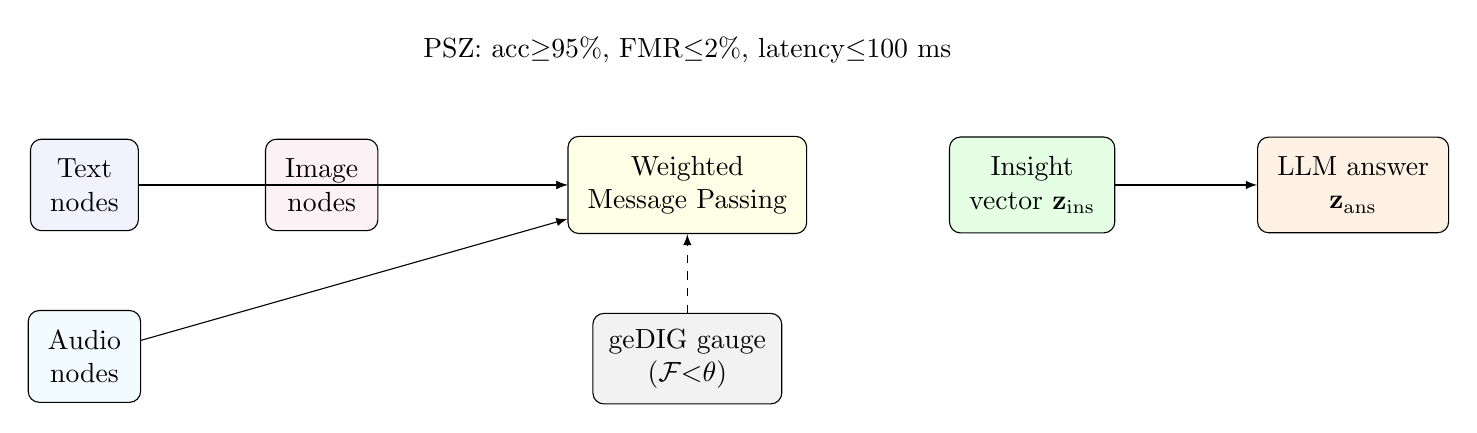
\begin{tikzpicture}[node distance=12mm, >=latex]
    \node[draw, rounded corners, align=center, inner sep=2.5mm, fill=blue!5] (txt) {Text\\nodes};
    \node[draw, rounded corners, align=center, inner sep=2.5mm, fill=purple!5, right=16mm of txt] (img) {Image\\nodes};
    \node[draw, rounded corners, align=center, inner sep=2.5mm, fill=cyan!5, below=10mm of txt] (aud) {Audio\\nodes};
    \node[draw, rounded corners, align=center, inner sep=2.5mm, fill=yellow!10, right=24mm of img] (mp) {Weighted\\Message Passing};
    \draw[->] (txt) -- (mp);
    \draw[->] (img) -- (mp);
    \draw[->] (aud) -- (mp);
    \node[draw, rounded corners, align=center, inner sep=2.5mm, fill=green!10, right=18mm of mp] (zins) {Insight\\vector $\mathbf{z}_{\mathrm{ins}}$};
    \node[draw, rounded corners, align=center, inner sep=2mm, fill=gray!10, below=10mm of mp] (gauge) {geDIG gauge\\($\mathcal{F}{<}\theta$)};
    \draw[->, dashed] (gauge) -- (mp);
    \node[draw, rounded corners, align=center, inner sep=2.5mm, fill=orange!10, right=18mm of zins] (llm) {LLM answer\\$\mathbf{z}_{\mathrm{ans}}$};
    \draw[->] (zins) -- (llm);
    \node[align=center, above=8mm of mp] (psz) {PSZ: acc$\ge$95\%, FMR$\le$2\%, latency$\le$100 ms};
  \end{tikzpicture}
  \caption{潜在言語空間上の世界モデル概念図。知識ノード(テキスト/画像/音声)を統一空間に正規化し,重み付きメッセージパッシングで言語ベクトル推論($\mathbf{z}_{\mathrm{ins}}$)を構成,geDIG を単一ゲージとして更新・計画を制御する。PSZ で運用の安全域を担保。}
  \label{fig:world_model_overview}
\end{figure}

% (English limitations removed; Japanese limitations above incorporate the same content.)

\section*{付録A. 命題の詳細と追加実験}

\subsubsection*{A.1 命題の詳細($\mathcal{F}\propto\Delta\mathrm{MDL}$)}
記述長 $\mathrm{MDL}(M,D)=L(M)+L(D\mid M)$ を、構造操作(置換=削除+挿入で上界化)と、観測の不確実性の減少で1次近似する。
\begin{align*}
 L(M) &\approx c_M\,\Delta\mathrm{GED}_{\mathrm{norm}},\\
 L(D\mid M) &\approx c_D\,\bigl(1-\Delta\mathrm{IG}_{\mathrm{norm}}\bigr),
\end{align*}
ここで $\Delta\mathrm{GED}_{\mathrm{norm}}\in[0,1]$、$\Delta\mathrm{IG}_{\mathrm{norm}}\in[-1,1]$ は無次元化済み(スケール整合)。差分を取れば
\begin{align*}
 \Delta\mathrm{MDL} &\approx c_M\,\Delta\mathrm{GED}_{\mathrm{norm}} - c_D\,\Delta\mathrm{IG}_{\mathrm{norm}} + \text{const.}
\end{align*}
比例係数 $\lambda=c_D/c_M$ を選ぶと $\mathcal{F}=\Delta\mathrm{GED}_{\mathrm{norm}}-\lambda\,\Delta\mathrm{IG}_{\mathrm{norm}}\propto\Delta\mathrm{MDL}$。誤差項は(i)置換の上界化、(ii)エントロピー推定の有限標本誤差、(iii)多ホップ有限和近似(\S2.3 の上界)から生じる。運用上は分位ベースの閾値校正で安定化する。

\subsubsection*{A.2 追加実験・旧稿ログ}
\begin{itemize}[leftmargin=*]
  \item \textbf{瞬間 $\Delta$GED の高速検出}: 初期稿では Hard=100\%、平均37ms でスパイク検出を実現。現稿の無次元化・多ホップ規約に写像可能。
  \item \textbf{E-geDIG の構想}: エッジ一次の line-graph 上で $\mathcal{F}_e=\Delta\mathrm{GED}_{\mathrm{edge}}-\lambda \Delta\mathrm{IG}_{\mathrm{edge}}$ を定義し、回路アセンブリの成立判定に応用可能。
\end{itemize}

\bibliographystyle{plain}
\bibliography{references}

\end{document}
